\section{Lista 2: Filtragem Linear Ótima} % <-----------------------------------------------------------------------------


\subsection{Filtragem Ótima} % <-----------------------------------------------------------------------------


\subsubsection*{Coeficientes de Wiener} % <-----------------------------------------------------------------------------

Considerando o problema de filtragem de Wiener, e assumindo conhecimento da matriz de correlação $\mathbf{R_{X}}$ e do vetor de correlação cruzada $\mathbf{p}_{\mathbf{X} d}$, pode-se obter os coeficientes de $\mathbf{w}$.
\begin{equation} 
    \mathbf{w} = \mathbf{R_{X}}^{-1} \mathbf{p}_{\mathbf{X} d} \label{eq:hw2p1}
\end{equation}

Aplicando a equação~\ref{eq:hw2p1}, obtém-se o vetor de pesos do filtro.
\begin{equation*}
    \mathbf{R_{X}}^{-1} =  \left[ \begin{matrix} 1.3333 & -0.6667 \\ -0.6667 & 1.3333 \end{matrix} \right]
\end{equation*}

\begin{align*} 
    \mathbf{w} &= \left[ \begin{matrix} 1.3333 & -0.6667 \\ -0.6667 & 1.3333 \end{matrix} \right] \left[ \begin{matrix} 0.5 \\ 0.25 \end{matrix} \right] \\
        &= \left[ \begin{matrix} 0.5 \\ 0 \end{matrix} \right] \, .
\end{align*}


\subsubsection*{Erro Médio Quadrático}

A partir do vetor de pesos, resultado de~\ref{eq:hw2p1}, basta aplicá-lo na equação do erro mínimo.
\begin{equation}
    \mathbb{E}\{e^{2}(n)\}  =\sigma^{2}_{d} - 2\mathbf{w}^{\top}\mathbf{p}_{\mathbf{X} d} + \mathbf{w}^{\top} \mathbf{R_{X}} \mathbf{w}      
\end{equation}
\begin{align*}
     e &= \sigma^{2}_{d} - 2 \left[ \begin{matrix} 0.5 & 0.0 \end{matrix} \right] \left[ \begin{matrix} 0.5 \\ 0.25 \end{matrix} \right] + \left[ \begin{matrix} 0.5 & 0.0 \end{matrix} \right] \left[ \begin{matrix} 1 & -0.5 \\ -0.5 & 1 \end{matrix} \right]  \left[ \begin{matrix} 0.5  \\ 0.0 \end{matrix} \right] \\
     &= \sigma^{2}_{d} - 2 \times 0.25 + 0.25 \\
     &= \sigma^{2}_{d} - 0.25
\end{align*}


\subsubsection*{Representação em Autovalores}
A decomposição em valores singulares (EVD) pode ser aplicada na matriz de correlação
\begin{equation}
    \mathbf{R}_{X} = \mathbf{Q} \mathbf{\Lambda} \mathbf{Q}^{-1} \label{eq:hw2p1_EVD}
\end{equation}


Aplicando diretamente o resultado da EVD~\ref{eq:hw2p1_EVD} na equação do filtro ótimo~\ref{eq:hw2p1}, obtém-se:
\begin{equation}
    \mathbf{w}= (\mathbf{Q} \mathbf{\Lambda} \mathbf{Q}^{-1})^{-1} \mathbf{p}_{\mathbf{X} d}
\end{equation}

Finalmente, o resultado é uma expressão que compreende a inversão de matrizes menos custosas computacionalmente. Isto se dá principalmente por $\mathbf{\Lambda}$ ser uma matriz diagonal contendo os autovalores da matriz de autocorrelação, bastando calcular $1/\lambda_{i}$ para obter a sua inversa.
\begin{equation}
    \mathbf{w} = \mathbf{Q}^{-1} \mathbf{\Lambda}^{-1} \mathbf{Q} \mathbf{p}_{\mathbf{X} d}.
\end{equation}
                                         

\subsection{Erro Médio Quadrático Mínimo} % <-----------------------------------------------------------------------------
Para verificar a expressão proposta, é necessário obter a matriz de correlação do vetor aumentado.
\begin{align*}
    \mathbf{A} &= \mathbb{E} \left\{ \left[ \begin{matrix} d(n) \\ x(n) \end{matrix} \right] \left[ \begin{matrix} d(n)^{\top} & x(n)^{\top} \end{matrix} \right] \right\} \\
    &= \left[ \begin{matrix} \mathbb{E}\{d(n) d(n)^{\top}\} & \mathbb{E}\{d(n) x(n)^{\top}\} \\ \mathbb{E}\{x(n) d(n)^{\top}\} & \mathbb{E}\{x(n) x(n)^{\top}\} \end{matrix} \right] \\
    &=  \left[ \begin{matrix} \sigma^{2}_{d} & \mathbf{p}_{\mathbf{X} d}^{\top} \\
        \mathbf{p}_{\mathbf{X} d} & \mathbf{R}_{X} \end{matrix} \right]
\end{align*}

É conveniente observar que ao desenvolver a equação, os elementos resultantes da expressão são todo conhecidos. Multiplicando o resultado obtido pelo vetor $\left[\begin{matrix}1 \\ -w \end{matrix} \right]$ à direita e assumindo o modelo nas condições de filtragem ótima, dado filtro de wiener, onde, $\mathbf{w}_{\text{opt}} = \mathbf{R}^{-1}_{X} \mathbf{p}_{\mathbf{X} d}$, temos que:

\begin{align*}
    \mathbf{A} \left[ \begin{matrix} 1 \\ -\mathbf{w} \end{matrix} \right] &= \left[ \begin{matrix} \sigma^{2}_{d} & \mathbf{p}_{\mathbf{X} d}^{\top} \\
        \mathbf{p}_{\mathbf{X} d} & \mathbf{R}_{X} \end{matrix} \right] \left[ \begin{matrix} 1 \\ -\mathbf{w} \end{matrix} \right] \\
        &=   \left[ \begin{matrix} \sigma^{2}_{d} - \mathbf{p}_{\mathbf{X} d}^{\top}\mathbf{w} \\ \mathbf{p}_{\mathbf{X} d} - \mathbf{R}_{X}\mathbf{w} \end{matrix} \right] \\
        &=   \left[ \begin{matrix} \sigma^{2}_{d} - \mathbf{p}_{\mathbf{X} d}^{\top}\mathbf{R}^{-1}_{X} \mathbf{p}_{\mathbf{X} d} \\
            \mathbf{p}_{\mathbf{X} d} - \mathbf{R}_{X}\mathbf{R}^{-1}_{X} \mathbf{p}_{\mathbf{X} d} \end{matrix} \right] \\
        &=   \left[ \begin{matrix} \sigma^{2}_{d} - \mathbf{p}_{\mathbf{X} d}^{\top}\mathbf{R}^{-1}_{X} \mathbf{p}_{\mathbf{X} d} \\
            \mathbf{p}_{\mathbf{X} d} - \mathbf{I}_{X}\mathbf{p}_{\mathbf{X} d} \end{matrix} \right] \\
        &=   \left[ \begin{matrix} \sigma^{2}_{d} - \mathbf{p}_{\mathbf{X} d}^{T
            }\mathbf{R}^{-1}_{X} \mathbf{p}_{\mathbf{X} d} \\ 0 \end{matrix} \right]
\end{align*}

Finalmente, dado a equação obtida, com expressão equivalente à $J_{min}$, pode-se escrever a relação proposta.
\begin{align*}
    \mathbf{A} \left[ \begin{matrix} 1 \\ -\mathbf{w} \end{matrix} \right] = \left[ \begin{matrix} J_{min} \\ 0 \end{matrix} \right]
\end{align*}


\subsection{Cancelamento de Ruído} % <-----------------------------------------------------------------------------

Formulando a expressão do erro a partir do sistema sugerido:
\begin{align*}
    e(n) &= x(n) - \hat{v_{1}} \\
    &= x(n) - \mathbf{w}^{T}v_{2}(n)
\end{align*}

Dado a equação obtida acima, deve-se aplicar: I) função erro quadrático médio (MSE), II) o operador valor esperado, com o filtro apresentando coeficientes constantes.

\begin{align*}
    \mathbb{E}\{e^{2}(n)\} &= \mathbb{E}\{x^{2}(n)\} - 2\mathbf{w}^{T}\mathbb{E}\{x(n) v_{2}(n)\} + \mathbf{w}^{T}\mathbb{E}\{v_{2}(n)v_{2}(n)^{T}\} \mathbf{w},& \\
    &= \sigma^{2}_{x} - 2\mathbf{w}^{T}\mathbf{p}_{xv_{2}} + \mathbf{w}^{T}\mathbf{R}_{v_{2}} \mathbf{w}.&
\end{align*}

Isto permite encontrar a equação para calculcar o $\mathbf{w}$ que minimiza o MSE via gradiante.

\begin{align*}
    \nabla_{\mathbf{w}} \mathbb{E}\{e^{2}(n)\} &= 0 \\
    - 2\mathbf{p}_{xv_{2}} + 2\mathbf{R}_{v_{2}} \mathbf{w} &= 0  \\
    -\mathbf{p}_{xv_{2}} + \mathbf{R}_{v_{2}} \mathbf{w} &= 0
\end{align*}

Por fim, temos que $\mathbf{w} = \mathbf{R}_{v_{2}}^{-1} \mathbf{p}_{xv_{2}}$ é o vetor de pesos do filtro.


\subsection{Predição Ótima} % <-----------------------------------------------------------------------------

O primeiro passo é definir a matriz de autocorrelação para $x(n)$. Visando a simplicidade, mas sem perda de generalidade, pode-se considerar que o processo $S$ é WSS e tem variância $\sigma^{2}_{s}$:
\begin{align*} 
    \mathbf{R}_{x} = 
    \begin{bmatrix}
        \mathbb{E}\{x(n)x^{*}(n)\} & \mathbb{E}\{x(n-1)x^{*}(n)\} \\
        \mathbb{E}\{x(n)x^{*}(n-1)\}  & \mathbb{E}\{x(n-1)x^{*}(n-1)\} 
    \end{bmatrix}
\end{align*}

Dado as premissas assumidas, a matriz pode ser simplificada para uma matriz diagonal preenchido por $2 \sigma^{2}_{s}$.

Finalmente, considerando média nula para o processo $D$, a consequencia é que o vetor de correlação cruzada também é nulo.


\begin{align*} 
    \mathbf{w}_{\text{opt}} &= \mathbf{R}^{-1}_{x} \mathbf{p}_{xd} \\
    & = 
    \begin{bmatrix}
        2 \sigma^{2}_{s} & 0 \\
        0  & 2 \sigma^{2}_{s}
    \end{bmatrix}
    \begin{bmatrix}
        0 \\
        0 
    \end{bmatrix} \\
    &= 
    \begin{bmatrix}
        0 \\
        0 
    \end{bmatrix}
\end{align*}

Isto implica que o filtro linear ótimo para esse processo seria o próprio vetor nulo.


\subsection{Superfície de Erro} % <-----------------------------------------------------------------------------

Dado os coeficientes, temos que a matriz de correlação $\mathbf{R}_{x}$ do filtro ótimo é uma matriz identidade de ordem $2 \times 2$.

Aplicando a solução do filtro ótimo de Wiener, obtém-se finalmente o vetor de pesos:
\begin{align*}
    \mathbf{w}_{\text{opt}} &= \mathbf{R}^{-1}_{x} \mathbf{p}_{xd} \\
    &= \left[ \begin{matrix} 1 & 0 \\ 0 & 1 \end{matrix} \right]  \left[ \begin{matrix} 2 \\ 4.5 \end{matrix} \right] \\
    &= \left[ \begin{matrix} 2 \\ 4.5 \end{matrix} \right]
\end{align*}


\textbf{A superfície definida por $J(\mathbf{w})$}

Abrindo a equação do erro médio, para obter a expressãoque define a superfície. 

\begin{align}
    \mathbf{J}(w) &= \mathbb{E}\{e^{2}(n)\} \\
    &= \sigma^{2}_{d} - 2\mathbf{w}^{T}\mathbf{p}_{xd} + w^{T}\mathbf{R}_{X}\mathbf{w}. \label{eq:mse}   
\end{align}

Aplicando os valores obtidos na expressão da superfície:
\begin{align*}
    \mathbf{J}(w_{0}, w_{1}) &= 24.40 - 2 \left[ \begin{matrix} w_{0}  w_{1} \end{matrix} \right] \left[ \begin{matrix} 2 \\ 4.5 \end{matrix} \right] + \left[ \begin{matrix} w_{0}  w_{1} \end{matrix} \right] \left[ \begin{matrix} 1 & 0 \\ 0 & 1 \end{matrix} \right]  \left[ \begin{matrix} w_{0}  \\ w_{1} \end{matrix} \right] \\
    &= 24.40 - 4w_{0} - 9w_{1} + w^{2}_{0} + w^{2}_{1}
\end{align*}

Utilizando um MATLAB é possível obter a Figura~\ref{fig:hw2p5} onde é traçada a superfície de erro MSE expressada na Equação (\ref{eq:mse}).

\begin{figure}[!htb]
    \centering
    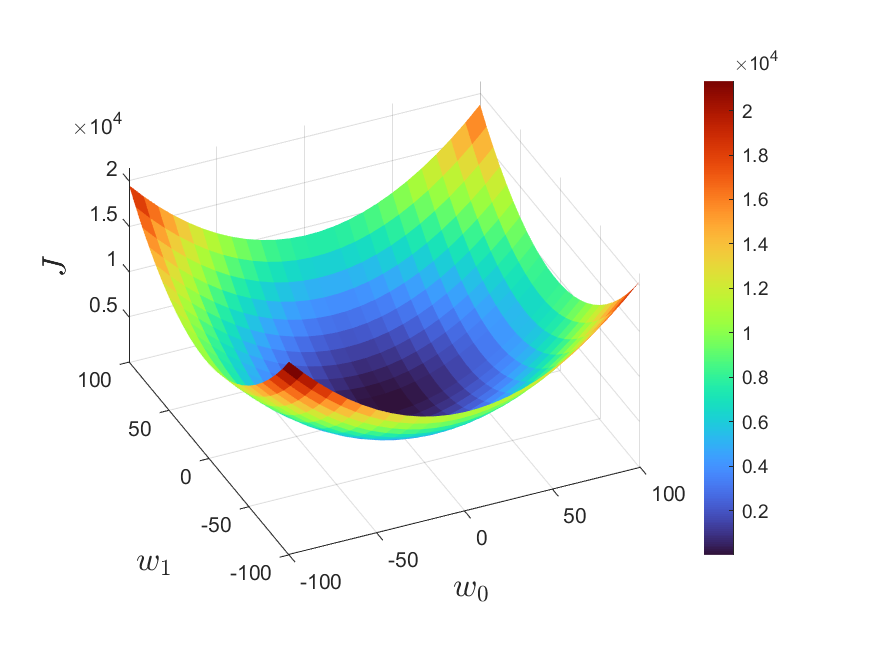
\includegraphics[width=1.0\textwidth]{C:/Users/lucasabdalah-dell/Documents/GitHub/Courses-HWs/Master/TIP7188-FILTRAGEM_ADAPTATIVA/homework/code/figures/hw2p5.pdf}
    \caption{Superfície de erro $J(w_{0}, w_{1})$.}
    \label{fig:hw2p5}
\end{figure}